\chapter{離散時間フィルタ}
    離散時間フィルタは次の通り分類される。
    \begin{enumerate}
        \item feedforward フィルタ\\
        出力がそれ以前の出力に依存しない。ディジタル計算機で実現するため,インパルス応答の長さは有限であると約束する。
        \item feedback フィルタ\\
        出力がそれ以前の出力に依存する。実用上の意味のあるフィルタは多くの場合 feedforward 構造を含み,そこに入力信号が入る。
        インパルス応答の長さは無限である場合が多いが,有限の場合もある(例えば CIC フィルタ)。
    \end{enumerate}
    \section{連続時間系のフィルタ処理を離散時間系で観測したときの振る舞い}
    ここでは,連続時間系でフィルタ処理を行った結果を離散時間系で観測したときの振る舞いを考える。
    この問題は実用上興味深い。
    物理系の状態をセンサでコンピュータに取り込み,有益な計算をする状況がこれに当てはまる。
    具体的には,無線受信機の直交分離出力であるIQ信号(連続時間信号)をADCで一定周期でサンプリングしてCPUに取り込んで復調の計算を行う状況が考えられる。
    \begin{shadebox}
        $h:\realNumbers\to\realNumbers$を連続時間信号とする。
        $H:\complexNumbers\to\complexNumbers$を$h$のLaplace変換とする。
        インパルス応答が$h$である連続時間フィルタを連続時間系の複素正弦波信号$x(t) = A\exp i(\omega_0 t + \phi)\;(A>0,\omega_0,\phi\in\realNumbers)$に適用した出力を$y=h*x$とする。
        $x,y$をサンプリング周期$\Ts$でサンプリングした離散時間信号を$\xd: n\in\integers\mapsto x(n\Ts), \yd: n\in\integers\mapsto y(n\Ts)$とする。
        このとき次式が成り立つ。
        \[ \DTFTwithArg{\yd}{\bm{\omega}} = H(i\omega_0)\DTFTwithArg{\xd}{\bm{\omega}} \]
    \end{shadebox}
    \begin{proof}
        \begin{align*}
            \DTFTwithArg{\yd}{\bm{\omega}} &= \sum_{m=-\infty}^\infty y(n\Ts)\exp \left(-i n\Ts\omega\right) = \sum_{m=-\infty}^\infty (h*x)(n\Ts)\exp \left(-i n\Ts\omega\right) \\
            &= \sum_{m=-\infty}^\infty \left(\integrate{-\infty}{\infty}{h(\tau)x(n\Ts-\tau)}{}{\tau}\right)\exp \left(-i n\Ts\omega\right) \\
            &= \integrate{-\infty}{\infty}{h(\tau)\sum_{m=-\infty}^\infty x(n\Ts-\tau)\exp \left(-i n\Ts\omega\right)}{}{\tau} \\
            &= \integrate{-\infty}{\infty}{h(\tau)\sum_{m=-\infty}^\infty A\exp i(\omega_0 (n\Ts-\tau) + \phi)\exp \left(-i n\Ts\omega\right)}{}{\tau} \\
            &= \integrate{-\infty}{\infty}{h(\tau) \exp(-i\omega_0\tau)\sum_{m=-\infty}^\infty A\exp i(\omega_0 n\Ts + \phi)\exp \left(-i n\Ts\omega\right)}{}{\tau} \\
            &= \DTFTwithArg{\xd}{\omega} \integrate{-\infty}{\infty}{h(\tau) \exp(-i\omega_0\tau)}{}{\tau} = \DTFTwithArg{\xd}{\omega}H(i\omega_0)
        \end{align*}
    \end{proof}
    \section{feedback フィルタの出力値の範囲}
    \newcommand{\Nff}{{N_{\text{ff}}}}
    \newcommand{\Nfb}{{N_{\text{fb}}}}
    \newcommand{\hInit}[1]{{h_{\text{init},#1}}}
    \newcommand{\HInit}[1]{{H_{\text{init},#1}}}
    \newcommand{\Minit}[1]{{M_{\text{init},#1}}}
    feedback フィルタの入力の絶対値が制限されるときの出力の絶対値の最大値を求める。
    この関係は feedback フィルタを実装する際に,内部の記憶素子と演算素子に必要なビット幅を決める際に役立つ。
    ここでは拡張性を重視して信号の終域を $\complexNumbers$ としているが,用途に応じて $\realNumbers$ に制限してもよい。
    \begin{shadebox}
        F を安定な feedback フィルタとし,$x,\;y:\integers\to\complexNumbers$ をそれぞれ入力と出力とする。
        $x$ は負の時刻に於いて 0 であり,全ての時刻に於いて絶対値が $M_x(\geq 0)$ 以下であるとする。
        F の漸化式が次式であるとする。
        \[ y(n) = \sum_{k=0}^\Nff a_k x(n-k) - \sum_{l=1}^\Nfb b_l y(n-l) \]
        ここに $\Nff,\;\Nfb\in\naturalNumbers$ はそれぞれ feedforward 経路、feedback 経路のタップ数であり, $a_k,\;b_l\in\complexNumbers$ は係数である。
        \par
        $h:\integers\to\complexNumbers$ を F の因果的なインパルス応答とし,$\hInit{l}:\integers\to\complexNumbers$ を次式の逆片側 Z 変換とする。
        \[ \frac{\sum_{k=l}^\Nfb b_{k} z^{-(k-l)}}{1+\sum_{k=1}^\Nfb b_k z^{-k}} \]
        $\Minit{l}\coloneq\max_n {\abs{\hInit{l}(n)}}$ とする。
        $y$ の値の範囲について次式が成り立つ。
        \[ \max_{n\in\naturalNumbers\cup\{0\}}\abs{y(n)} \leq M_x\sum_{k=0}^\infty\abs{h(k)} + \sum_{l=1}^\Nfb\abs{y(-l)}\Minit{l} \]
        とくに,負の時刻について $y$ の値が 0 であるならば次式が成り立つ。
        \[ \max_{n\in\naturalNumbers\cup\{0\}}\abs{y(n)} \leq M_x\sum_{k=0}^\infty\abs{h(k)} \]
    \end{shadebox}
    \begin{proof}
        \quad\par
        漸化式の両辺を片側 Z 変換して次式を得る。
        \begin{align*}
            Y(z) &= \parens*{\sum_{k=0}^\Nff a_k z^{-k}}X(z) - \sum_{l=1}^\Nfb b_l z^{-l}\parens*{\sum_{m=1}^l y(-m)z^m + Y(z)} \\
            \parens*{1+\sum_{l=1}^\Nfb b_l z^{-l}}Y(z) &= \parens*{\sum_{k=0}^\Nff a_k z^{-k}}X(z) - \sum_{m=1}^\Nfb y(-m) \sum_{l=m}^\Nfb b_l z^{-(l-m)} \\
            Y(z) &= \frac{\sum_{k=0}^\Nff a_k z^{-k}}{1+\sum_{l=1}^\Nfb b_l z^{-l}}X(z) - \parens*{\sum_{m=1}^\Nfb y(-m)}\frac{\sum_{l=m}^\Nfb b_l z^{-(l-m)}}{1+\sum_{l=1}^\Nfb b_l z^{-l}} \\
            &= H(z)X(z) - \sum_{m=1}^\Nfb y(-m) \HInit{m}(z)
        \end{align*}
        ここに $H$ は F の伝達関数であり,$\HInit{m}$ は $\hInit{m}$ の片側 Z 変換である。
        上式の両辺を逆片側 Z 変換して次式を得る\footnote{$h,\;x$ はともに因果的であるから \ref{single_sided_Z_transform_of_convolution} の結果が使える}。
        \[ y(n) = (h*x)(n) - \sum_{m=1}^\Nfb y(-m) \hInit{m}(n) \quad \therefore\abs{y(n)} \leq \abs{(h*x)(n)} + \sum_{m=1}^\Nfb \abs{y(-m)} \Minit{m} \]
        右辺第 1 項を評価する。
        \begin{align*}
            \abs{(h*x)(n)} &= \abs{\sum_{k=-\infty}^\infty h(k)x(n-k)} \leq \sum_{k=-\infty}^\infty \abs{h(k)}\abs{x(n-k)} \leq \sum_{k=0}^n \abs{h(k)}M_x\;(\because \forall n<0,\; h(n)=x(n)=0) \\
            &\leq M_x\sum_{k=0}^\infty \abs{h(k)}
        \end{align*}
        以上より主張が成り立つ。
    \end{proof}
    \section{feedforward フィルタ係数の設計}
    \subsection{DTFT の誤差 2 乗積分最小化}
        \newcommand*{\Hideal}{H_\text{ideal}}
        \newcommand*{\vhOpt}{\bm{h}_\text{opt}}
        ここではフィルタ係数が複素数であり,個数が指定された条件下で,所望の周波数スペクトラムに対して DTFT の誤差の重み付き 2 乗積分が最小になるように係数を決定する方法を記す。
        \par
        この方法は係数の個数について偶奇を区別せず,係数の添え字に関する対称性も指定していないため,線形位相特性は保証されない(意図的に線形位相特性を狙う方法については \cite{learn_sp_from_basic} 「8.3.1 線形位相 FIR フィルタの設計法」に詳細がある)。
        周波数スペクトラムの補正のための逆特性フィルタの設計のように,所望のフィルタの周波数スペクトラムが必ずしも線形位相特性を持たない場面を想定している。
        \par
        この方法で作られたフィルタの振幅周波数スペクトラムにはリップルが生じる可能性がある(激しさは所望の周波数スペクトラムの不連続性の強さに依る)。
        その際の緩和策として \cite{learn_sp_from_basic} 「8.3.2 窓関数を用いた設計法」が適用できると期待される。
        \subsubsection{誤差の重みが一様である場合}
            \label{誤差の重みが一様である場合}
            \newcommand*{\Nm}{{N_\text{m}}}
            \newcommand*{\Np}{{N_\text{p}}}
            ここでは全ての周波数に於いて誤差の重みを 1 としたときの最適係数を導く。
            \begin{shadebox}
                $\Nm,\Np\in\naturalNumbers\cup\{0\}$ とする。
                $N\coloneq\Nm+\Np+1$ 個の複素数 $h_{-\Nm},h_{-\Nm+1},\dots,h_{\Np-1},h_\Np$ を係数とする feedforward フィルタを考える。
                $h_0$ はインパルス応答の時刻 0 に対応する(因果律に関する注意事項は \ref{因果的フィルタとして実現する方法} で述べられる)。
                この周波数スペクトラム(フィルタ係数列の DTFT)を $H:\realNumbers\to\complexNumbers$ と記し,所望の周波数スペクトラムを $\Hideal:\realNumbers\to\complexNumbers$ と記す。
                但し $H$ と $\Hideal$ の引数はサンプル周波数について正規化された角周波数である($\pi/2$ が Nyquist 周波数に対応する)。
                $\bm{h} \coloneq [h_{-\Nm},h_{-\Nm+1},\dots,h_{\Np-1},h_\Np]^\top$ として次式で定義される $H$ と $\Hideal$ の誤差 2 乗積分の評価関数
                \[ J(\bm{h}) \coloneq \frac{1}{2\pi}\integrate{-\pi}{\pi}{\abs{H(\Omega)-\Hideal(\Omega)}^2}{}{\Omega} \tag{1} \]
                の最小点 $\vhOpt$ の第 $n\in\naturalNumbers\cup\{0\}$ 要素は次式である。
                \[ \vhOpt[n] = \frac{1}{2\pi}\integrate{-\pi}{\pi}{\Hideal(\Omega)\NapierE^{i\Omega (n-\Nm)}}{}{\Omega} = \IDTFT{\Hideal}(n-\Nm) \]
                とくに $\Hideal$ が Hermite 対称であるとき(実数値信号の周波数スペクトラム)は $\vhOpt\in\realNumbers^N$ となる。
            \end{shadebox}
            \begin{proof}
                \quad\par\noindent
                (最小点の導出)
                \begin{align*}
                    J(\bm{h}) &= \frac{1}{2\pi}\integrate{-\pi}{\pi}{\parens*{H(\Omega)-\Hideal(\Omega)}\parens*{\conj{H(\Omega)-\Hideal(\Omega)}}}{}{\Omega} \\
                    &= \frac{1}{2\pi}\integrate{-\pi}{\pi}{\parens*{\sum_{k=-\Nm}^\Np h_k\NapierE^{-i\Omega k} -\Hideal(\Omega)}\parens*{\sum_{l=-\Nm}^\Np \conj{h_l}\NapierE^{i\Omega l} -\conj{\Hideal(\Omega)}}}{}{\Omega} \\
                    &= \frac{1}{2\pi}\sum_{k=-\Nm}^\Np\sum_{l=-\Nm}^\Np h_k\conj{h_l}\integrate{-\pi}{\pi}{\NapierE^{i\Omega(l-k)}}{}{\Omega} - \frac{1}{2\pi}\sum_{k=-\Nm}^\Np h_k\integrate{-\pi}{\pi}{\conj{\Hideal(\Omega)}\NapierE^{-i\Omega k}}{}{\Omega} \\
                    &\phantom{=}- \frac{1}{2\pi}\sum_{l=-\Nm}^\Np \conj{h_l}\integrate{-\pi}{\pi}{\Hideal(\Omega)\NapierE^{i\Omega l}}{}{\Omega} + \frac{1}{2\pi}\integrate{-\pi}{\pi}{\abs{\Hideal(\Omega)}^2}{}{\Omega} \\
                    &= \norm{\bm{h}}_2^2 - \frac{1}{2\pi}2\Re{\sum_{k=-\Nm}^\Np h_k\integrate{-\pi}{\pi}{\conj{\Hideal(\Omega)}\NapierE^{-i\Omega k}}{}{\Omega}} + \frac{1}{2\pi}\integrate{-\pi}{\pi}{\abs{\Hideal(\Omega)}^2}{}{\Omega} \tag{2}
                \end{align*}
                ここで $v_k\;(k=-\Nm,\;-\Nm+1,\;\dots,\;\Np)$ を次式で定義し,$\bm{v}\coloneq[v_{-\Nm},\;v_{-\Nm+1},\;\dots,\;v_\Np]^\top$ とする。
                \[ v_n \coloneq \frac{1}{2\pi}\integrate{-\pi}{\pi}{\Hideal(\Omega)\NapierE^{i\Omega n}}{}{\Omega} \]
                式 (2) の第 3 項は $\bm{h}$ に依存しないので無視し,第 2 項までを取り出して次の評価関数を得る。
                \[ J_2(\bm{h}) \coloneq \norm{\bm{h}}_2^2 - 2\Re{\bm{v}^*\bm{h}} = \norm{\bm{h} - \bm{v}}_2^2 - \norm{\bm{v}}_2^2 \]
                これの最小点が $\bm{v}$ であるから主張が従う。
                \newline
                \par\noindent
                ($\Hideal$ が Hermite 対称であるときは $\vhOpt\in\realNumbers^N$ となること)
                \[ \vhOpt[n] = \frac{1}{2\pi}\bracks*{\underbrace{\integrate{-\pi}{0}{\Hideal(\Omega)\NapierE^{i\Omega (n-\Nm)}}{}{\Omega}}_{(3)} + \integrate{0}{\pi}{\Hideal(\Omega)\NapierE^{i\Omega (n-\Nm)}}{}{\Omega}} \]
                式 (3) に変数変換を施すと次式を得る。
                \[ (3) = \integrate{0}{\pi}{\Hideal(-\Omega)\NapierE^{-i\Omega (n-\Nm)}}{}{\Omega} = \conj{\integrate{0}{\pi}{\Hideal(\Omega)\NapierE^{i\Omega (n-\Nm)}}{}{\Omega}} \]
                よって次式を得る。
                \[ \vhOpt[n] = \frac{1}{\pi}\Re{\integrate{0}{\pi}{\Hideal(\Omega)\NapierE^{i\Omega (n-\Nm)}}{}{\Omega}}\in\realNumbers \]
            \end{proof}
            \paragraph{因果的フィルタとして実現する方法}
                \label{因果的フィルタとして実現する方法}
                $\Nm>0$ のときは前記のフィルタ係数の添え字に負数が含まれ,因果的フィルタとして実現できない。
                最小の添え字が 0 になるように時間的にシフトする必要がある。
                フィルタの応答が時間的に遅れる(周波数領域に於いては遅れに比例した角周波数の複素指数関数が乗じられる)が,無線通信等の大抵の用途では問題にならない。
            \paragraph{Note:IDFT による係数設計との違い}
                \newcommand*{\kmin}{{k_\text{min}}}
                \newcommand*{\kmax}{{k_\text{max}}}
                \newcommand*{\HidealNA}{H_\text{ideal,NA}}
                実用の場面では $\Hideal$ が等間隔の離散的な正規化角周波数についてのみ得られることがある。
                その場合に $\bm{h}$ の決定によく用いられているのは IDFT である。
                IDFT による結果と \ref{誤差の重みが一様である場合} の結果が一般には一致しないことを示しておく。
                \par
                $\Delta f>0,\;\kmin,\;\kmax\in\integers,\;\kmax>\kmin$ とする。
                $\Hideal$ の値が $k\Delta f\;k=\kmin,\kmin+1,\dots,\kmax$ に関して得られているとする。
                $\Hideal$ の Fourier 変換の台が $[-1/(2\Delta f),1/(2\Delta f)]$ に含まれているものとする。
                標本化定理から次式が成り立つ。
                \[ \Hideal(f) = \sum_{k=\kmin}^\kmax \Hideal(k\Delta f)\sinc\frac{\pi}{\Delta f}(f-k\Delta f) \]
                サンプル周波数を $\fsamp$ として $\Hideal$ を正規化角周波数で表したものを $\HidealNA$ とすると次式を得る。
                \[ \HidealNA(\Omega) = \Hideal(\Omega\fsamp/(2\pi)) \]
                これに対して \ref{誤差の重みが一様である場合} の方法を適用すると次式が成り立つ。
                \begin{align*}
                    \vhOpt[n] &= \IDTFT{\HidealNA}(n-\Nm) = \sum_{k=\kmin}^\kmax \Hideal(k\Delta f)\IDTFT{\Omega\mapsto\sinc\frac{\pi}{\Delta f}\parens*{\frac{\Omega\fsamp}{2\pi}-k\Delta f}}(n-\Nm) \\
                    &= \sum_{k=\kmin}^\kmax \Hideal(k\Delta f)\frac{1}{2\pi}\integrate{-\pi}{\pi}{\bracks*{\sinc\frac{\pi}{\Delta f}\parens*{\frac{\Omega\fsamp}{2\pi}-k\Delta f}}(\exp i\Omega(n-\Nm))}{}{\Omega}
                \end{align*}
                これは一般には IDFT による結果と一致しない。
        \subsubsection{誤差の重みが一様ではない場合}
            ここでは,誤差の重みが周波数に依存する場合の最適係数を導く。
            \begin{shadebox}
                $w:\realNumbers\to\realNumbers$ は非負であり,$w>0$ となる区間が $[-\pi,\pi]$ に少なくとも 1 つ存在するものとする。
                式 (1) を変更し,次の評価関数を考える。
                \[ J(\bm{h}) \coloneq \frac{1}{2\pi}\integrate{-\pi}{\pi}{w(\Omega)\abs{H(\Omega)-\Hideal(\Omega)}^2}{}{\Omega}\tag{4} \]
                これの最小点 $\vhOpt$ は次式である。
                \[ \vhOpt = A^{-1}\bm{v} \]
                ここに $A\in\complexNumbers^{N\times N},\;\bm{v}\in\complexNumbers^N$ はそれぞれ次式で定義される。
                \[ A[m,n] \coloneq \frac{1}{2\pi}\integrate{-\pi}{\pi}{w(\Omega)\NapierE^{i\Omega(m-n)}}{}{\Omega},\quad v[m] \coloneq \frac{1}{2\pi}\integrate{-\pi}{\pi}{w(\Omega)\Hideal(\Omega)\NapierE^{i\Omega (m-\Nm)}}{}{\Omega} \]
                とくに $\Hideal$ が Hermite 対称であり(実数値信号の周波数スペクトラム),かつ $w$ が偶関数であるときは $\vhOpt\in\realNumbers^N$ となる。
            \end{shadebox}
            \begin{proof}
                \quad\par\noindent
                (最小点の導出)
                \par
                式 (1) と同じ要領で式変形を行うと次式を得る。
                \begin{align*}
                    J(\bm{h}) &= \frac{1}{2\pi}\integrate{-\pi}{\pi}{w(\Omega)\parens{H(\Omega)-\Hideal(\Omega)}\parens{\conj{H(\Omega)-\Hideal(\Omega)}}}{}{\Omega} \\
                    &= \frac{1}{2\pi}\sum_{k=-\Nm}^\Np\sum_{l=-\Nm}^\Np h_k\conj{h_l}\integrate{-\pi}{\pi}{w(\Omega)\NapierE^{i\Omega(l-k)}}{}{\Omega} - \frac{1}{2\pi}2\Re{\sum_{k=-\Nm}^\Np h_k\integrate{-\pi}{\pi}{w(\Omega)\conj{\Hideal(\Omega)}\NapierE^{-i\Omega k}}{}{\Omega}} \\
                    &\phantom{=} + \frac{1}{2\pi}\integrate{-\pi}{\pi}{w(\Omega)\abs{\Hideal(\Omega)}^2}{}{\Omega}\tag{5}
                \end{align*}
                $N\times N$ Hermite 対称行列 $A$ を,第 $(l,k)$ 要素が次式で定義されるものとする。
                \[ A[l,k] \coloneq \frac{1}{2\pi}\integrate{-\pi}{\pi}{w(\Omega)\NapierE^{i\Omega((l-\Nm)-(k-\Nm))}}{}{\Omega} = \frac{1}{2\pi}\integrate{-\pi}{\pi}{w(\Omega)\NapierE^{i\Omega(l-k)}}{}{\Omega} \]
                また $v_n\;(n=-\Nm,\;-\Nm+1,\;\dots,\;\Np)$ を次式で定義し,$\bm{v}\coloneq[v_{-\Nm},\;v_{-\Nm+1},\;\dots,\;v_\Np]^\top$ とする。
                \[ v_n \coloneq \frac{1}{2\pi}\integrate{-\pi}{\pi}{w(\Omega)\Hideal(\Omega)\NapierE^{i\Omega n}}{}{\Omega} \]
                上記を式 (5) に適用し,$\bm{h}$ に依存しない項を無視すると次の評価関数を得る。
                \[ J_2(\bm{h}) \coloneq \bm{h}^*A\bm{h} - 2\Re{\bm{v}^*\bm{h}} \]
                証明していないが $A$ は正定値であると期待され\footnote{$w$ が偶関数であれば,区間 $[-\pi,\pi]$ に於ける $w$ の Fourier 級数展開を考えると $A$ が巡回行列となって固有値が容易に計算でき,正定性を示せるように思える。試してはいない。},以下ではそう仮定する。
                すると $J_2(\bm{h})$ は $\bm{h}$ の狭義凸 2 次形式であり,最小点が存在する。
                それは $\bm{h}$ が微小量 $\Delta\bm{h}$ 変化するときの $J_2$ の増分 $\Delta J_2(\bm{h})$ が 0 となる $\bm{h}$ である。
                \[ \Delta J_2(\bm{h}) = \bm{h}^*A\Delta\bm{h} + \Delta\bm{h}^*A\bm{h} - 2\Re{\bm{v}^*\Delta\bm{h}} + \underset{\norm{\Delta\bm{h}}_2\to 0}{o}(\norm{\Delta\bm{h}}_2) = 2\Re{(\bm{h}^*A-\bm{v}^*)\Delta\bm{h}} \]
                $\Delta J_2(\bm{h}) = 0\iff\bm{h} = A^{-1}\bm{v}$ であるから主張が従う。
                \newline
                \par\noindent
                ($\Hideal$ が Hermite 対称であり(実数値信号の周波数スペクトラム),かつ $w$ が偶関数であるときは $\vhOpt\in\realNumbers^N$ となること)
                \par
                重みが一様である場合 (\cref{誤差の重みが一様である場合}) の導出と同じ要領で $A\in\realNumbers^{N\times N},\;\bm{v}\in\realNumbers^N$ であることが容易に示せて $\vhOpt=A^{-1}\bm{v}\in\realNumbers^N$ である。
            \end{proof}
    \subsection{DTFT の誤差の実部と虚部の∞ノルム最小化}
        \newcommand*{\Ntp}{N_{\text{tp}}}
        \newcommand*{\Hid}{H_{\text{id}}}
        \newcommand*{\HidR}{H_{\text{id,r}}}
        \newcommand*{\HidI}{H_{\text{id,i}}}
        \newcommand*{\HidH}{H_{\text{id,H}}}
        \newcommand*{\HidHr}{H_{\text{id,H,r}}}
        \newcommand*{\HidHi}{H_{\text{id,H,i}}}
        \newcommand*{\HidSH}{H_{\text{id,SH}}}
        \newcommand*{\HidSHr}{H_{\text{id,SH,r}}}
        \newcommand*{\HidSHi}{H_{\text{id,SH,i}}}
        \newcommand*{\hes}{h_{\text{es}}}
        \newcommand*{\hos}{h_{\text{os}}}
        \newcommand*{\Hes}{H_{\text{es}}}
        \newcommand*{\Hos}{H_{\text{os}}}
        \newcommand*{\hr}{h_{\text{r}}}
        \newcommand*{\hi}{h_{\text{i}}}
        \newcommand*{\hrEs}{h_{\text{r,es}}}
        \newcommand*{\hrOs}{h_{\text{r,os}}}
        \newcommand*{\hiEs}{h_{\text{i,es}}}
        \newcommand*{\hiOs}{h_{\text{i,os}}}
        \newcommand*{\hesOpt}{h_{\text{es,opt}}}
        \newcommand*{\hosOpt}{h_{\text{os,opt}}}
        \newcommand*{\hopt}{h_{\text{opt}}}
        \newcommand*{\hrEsOpt}{h_{\text{r,es,opt}}}
        \newcommand*{\hrOsOpt}{h_{\text{r,os,opt}}}
        \newcommand*{\hiEsOpt}{h_{\text{i,es,opt}}}
        \newcommand*{\hiOsOpt}{h_{\text{i,os,opt}}}
        \newcommand*{\HesOpt}{H_{\text{es,opt}}}
        \newcommand*{\HosOpt}{H_{\text{os,opt}}}
        \newcommand*{\Hopt}{H_{\text{opt}}}
        \newcommand*{\HrEsOpt}{H_{\text{r,es,opt}}}
        \newcommand*{\HrOsOpt}{H_{\text{r,os,opt}}}
        \newcommand*{\HiEsOpt}{H_{\text{i,es,opt}}}
        \newcommand*{\HiOsOpt}{H_{\text{i,os,opt}}}
        \newcommand*{\eEs}{\mathrm{e}_{\text{es}}}
        \newcommand*{\eOs}{\mathrm{e}_{\text{os}}}
        \newcommand*{\eOpt}{\mathrm{e}_{\text{opt}}}
        \newcommand*{\erEs}{\mathrm{e}_{\text{r,es}}}
        \newcommand*{\erOs}{\mathrm{e}_{\text{r,os}}}
        \newcommand*{\eiEs}{\mathrm{e}_{\text{i,es}}}
        \newcommand*{\eiOs}{\mathrm{e}_{\text{i,os}}}
        フィルタ係数が複素数であり,個数が指定された条件下で,所望の周波数スペクトラムに対して DTFT の誤差の実、虚部それぞれの偶、奇対称成分の $L^\infty$-ノルムが最小になるように係数を決定する方法を記す。
        $H$ が線形位相特性をもち,かつ偶対称か奇対称のいずれかである場合(★ 1)には Remez のアルゴリズムが知られている(例えば \cite{DSP_JL} の \inlineCode{remez} 関数)。
        ここでは $H$ が★ 1 の条件を満たさない場合にも Remez のアルゴリズムを 4 回独立に実行してフィルタ係数を決定する方法を示す。
        また特殊ケースとして,入力信号が実数(従ってフィルタ係数も実数)である場合に Remez のアルゴリズムを 2 回独立に実行してフィルタ係数を決定する方法も示す。
        議論の見通しを良くするため,まず特殊ケースを導き,これを拡張して最終的な結論を導く。
        \subsubsection{前提}
            以下では周波数スペクトラムの補償用フィルタのように, null を含まない穏やかな特性を持つフィルタを主な関心の対象としている。
            そのため以下ではフィルタ係数の個数 $\Ntp\in\naturalNumbers$ は奇数であるとする。
            そうでない場合も以下で述べる手法がそのまま使える。
        \subsubsection{信号が実数の場合}
            まず信号が実数であり,従ってフィルタ係数も実数である場合について述べる。
            入力信号が実数であるから $\Hid$ は Hermite 対称である。
            \paragraph{偶、奇対称の係数がもたらす周波数スペクトラム}
                \label{偶、奇対称の係数がもたらす周波数スペクトラム}
                Remez のアルゴリズムの適用を考える準備として,添え字に関して偶対称と奇対称な係数がもたらす周波数スペクトラムを見ておく。
                いま,$\hes:\integers\to\realNumbers$ と $\hos:\integers\to\realNumbers$ をそれぞれ次式を満たす偶対称と奇対称(「対称」とは,中央の係数を中心にして言う)のフィルタ係数であって,係数列の長さが $\Ntp\in\naturalNumbers$ であるとする。
                \begin{align*}
                    \hes(m) &= \begin{cases}
                        \hes(\Ntp-1-m) & \parens*{m =0,1,\dots,(\Ntp-1)/2} \\
                        0 & (\text{otherwise})
                    \end{cases} \\
                    \hos(m) &= \begin{cases}
                        -\hos(\Ntp-1-m) & \parens*{m =0,1,\dots,(\Ntp-1)/2} \\
                        0 & (\text{otherwise})
                    \end{cases}
                \end{align*}
                (上の条件から $\hos((\Ntp-1)/2) = 0$ である。)
                \par
                $\Hes,\;\Hos$ をそれぞれ $\hes,\;\hos$ に対応する周波数スペクトラムとする(但し引数は正規化角周波数)と,簡単な計算を経て次式を得る。
                \begin{align*}
                    \Hes(\Omega) &= \exp\parens*{-i\frac{\Ntp-1}{2}\Omega}\bracks*{\hes\parens*{\frac{\Ntp-1}{2}} + 2\sum_{m=0}^{(\Ntp-1)/2-1}{\hes(m)\cos\Omega\parens*{\frac{\Ntp-1}{2}-m}}} \\
                    \Hos(\Omega) &= 2i\exp\parens*{-i\frac{\Ntp-1}{2}\Omega}\sum_{m=0}^{(\Ntp-1)/2-1}{\hos(m)\sin\Omega\parens*{\frac{\Ntp-1}{2}-m}}
                \end{align*}
                両者とも線形位相特性である(その和については一般にそうならない)。
                さらに $\Hos$ は $\Hes$ に比べて位相が $\pi/2$ だけ進んでいる。
                $\exp\parens*{-i\frac{\Ntp-1}{2}\Omega}$ は因果律を満たすためにフィルタ係数の 0 番目の添え字の位置を時刻の基準にとった為の位相の線形な遅れである。
                後述する Remez のアルゴリズムはこのような線形な位相遅れの部分が取り除かれた実数値関数を引数として受け取るため,適切に配慮すれば問題ない。
                この位相遅れの部分を無視すれば $\Hes$ は偶対称,$\Hos$ は奇対称である。
            \paragraph{Remez のアルゴリズムによる係数の決定}
                \label{Remez のアルゴリズムによる係数の決定}
                $\Hid$ の実部と虚部をそれぞれ $\HidR,\;\HidI$ とする。
                $\Hid$ が Hermite 対称であるから $\HidR$ は偶対称,$i\HidI$ は奇対称である。
                \ref{偶、奇対称の係数がもたらす周波数スペクトラム} の考察に従って $\HidR,\;i\HidI$ をそれぞれ近似する偶対称と奇対称の係数を求めればよいと解る。
                \par
                \cite{DSP_JL} の \inlineCode{remez} 関数は近似対象の周波数スペクトラムとして偶対称と奇対称の実数値関数の両方を扱える(\inlineCode{neg} オプションで選択)。
                さらにその関数をユーザが定義した関数オブジェクトで指定できる。
                実装の都合上,奇対称の周波数スペクトラムを与えて得られる出力は実数係数であるが,これを DTFT すると,偶対称の周波数スペクトラムから得られる出力に比べて位相が $\pi/2$ 進んだ結果になる。
                つまり \inlineCode{remez} 関数に $\HidI$ を与えて得られる係数の DTFT が近似するのは $\HidI$ ではなく $i\HidI$ である。
                \par
                上記の \inlineCode{remez} 関数を使って $\HidR,\;i\HidI$ を近似する係数 $\hesOpt,\;\hosOpt:\integers\to\realNumbers$ が求まる。
                両者の和 $\hopt \coloneq \hesOpt + \hosOpt$ が所望の係数である。
                \par
                $\hesOpt,\;\hosOpt,\;\hopt$ に対応する周波数スペクトラムをそれぞれ $\HesOpt,\;\HosOpt,\;\Hopt$ とする($\HosOpt(\Omega)\in i\realNumbers$ に注意)。
                $\hesOpt,\;\hosOpt,\;\hopt$ の近似誤差,即ち次式で表される $L^\infty$-ノルム
                \begin{align*}
                    \eEs &\coloneq \Verts{\HesOpt - \HidR}_\infty = \max_{\Omega\in[-\pi,\pi]}\abs{\HesOpt(\Omega) - \HidR(\Omega)} \\
                    \eOs &\coloneq \Verts{\HosOpt - i\HidI}_\infty = \max_{\Omega\in[-\pi,\pi]}\abs{\HosOpt(\Omega) - i\HidI(\Omega)} \\
                    \eOpt &\coloneq \Verts{\Hopt - \Hid}_\infty = \max_{\Omega\in[-\pi,\pi]}\abs{\Hopt(\Omega ) -\Hid(\Omega)}
                \end{align*}
                に三角不等式を適用して次式を得る。
                \[ \eOpt = \Verts{\Hopt - \Hid}_\infty = \Verts{\HesOpt - \HidR + (\HosOpt - i\HidI)}_\infty \leq \eEs + \eOs \]
                Remez のアルゴリズム 1 回分の誤差の高々 2 倍程度に収まる。
        \subsubsection{信号が複素数の場合}
            フィルタ係数も複素数であるとする。
            このときは $\Hid$ は Hermite 対称とは限らないが,次のように Hermite 対称、歪 Hermite 対称 (Skew-Hermitian) な 2 つの関数 $\HidH,\;\HidSH$ の和に分解できる。
            \begin{gather*}
                \Hid(\Omega) = \HidH(\Omega) + \HidSH(\Omega) \\
                \text{where}\quad\HidH(\Omega)\coloneq\frac{1}{2}\parens*{\Hid(\Omega) + \conj{\Hid(-\Omega)}},\quad\HidSH(\Omega)\coloneq\frac{1}{2}\parens*{\Hid(\Omega) - \conj{\Hid(-\Omega)}}
            \end{gather*}
            $\HidH$ の実部と虚部をそれぞれ $\HidHr,\;\HidHi$ とすると前者は偶対称,後者は奇対称である。
            また $\HidSH$ の実部と虚部をそれぞれ $\HidSHr,\;\HidSHi$ とすると前者は奇対称,後者は偶対称である。
            これら 4 つに対して Remez のアルゴリズムを使って,近似するためのフィルタ係数(実数値)を求めて(適宜,虚数単位を掛けながら)和をとれば所望の係数となる。
            \par
            設計するフィルタ係数を $h:\integers\to\realNumbers$ とし,それらの実部と虚部をそれぞれ $\hr,\;\hi$ とする。
            $\hr$ によって $\HidH$ を近似し,$\hi$ によって $\HidSH$ を近似する。
            \par
            $\hr$ を偶対称、奇対称な 2 つの成分に分解し,それぞれを $\hrEs,\;\hrOs$ とする。
            この分解は常に可能である。具体的には $\hr$ とその左右反転の和の 1/2 倍を $\hrEs$ とし,$\hr$ とその左右反転の差の 1/2 倍を $\hrOs$ とすればよい。
            $\hrEs,\;\hrOs$ については \ref{Remez のアルゴリズムによる係数の決定} と同じ方法で最適値 $\hrEsOpt,\;\hrOsOpt$ が求まる。
            \par
            次に $\hi$ の最適値を求める。
            $\hi$ を偶対称、奇対称な 2 つの成分に分解し,それぞれを $\hiEs,\;\hiOs$ とする。
            天下り的であるが(妥当性は以降の解説で直ぐに解る) Remez のアルゴリズムを使って $\hiEs$ によって $\HidSHi$ を近似して最適値を $\hiEsOpt$ とし,$\hiOs$ によって $-i\HidSHr$ を近似して最適値を $\hiOsOpt$ とする。
            \par
            $\hrEsOpt,\;\hrOsOpt,\;\hiEsOpt,\;\hiOsOpt$ に対応する周波数スペクトラムを $\HrEsOpt,\;\HrOsOpt,\;\HiEsOpt,\;\HiOsOpt$ とする($\HrOsOpt(\Omega),\;\HiOsOpt(\Omega)\in i\realNumbers$ に注意)。
            最終的な最適係数は $\hopt = \hrEsOpt + \hrOsOpt + i(\hiEsOpt + \hiOsOpt)$ である。
            それに対応する周波数スペクトラム $\Hopt$ は次式である。
            但し因果律を満たすために生じる位相遅れ $\exp\parens*{-i\frac{\Ntp-1}{2}\Omega}$ は無害であるから無視する。
            \begin{align*}
                \Hopt &= \HrEsOpt + \HrOsOpt + i(\HiEsOpt + \HiOsOpt) = \HrEsOpt + \HrOsOpt + i\HiEsOpt + i\HiOsOpt \\
                &\approx \HidHr + i\HidHi + i\HidSHi + \HidSHr = \Hid
            \end{align*}
            $\hrEsOpt,\;\hrOsOpt,\hiEsOpt,\;\hiOsOpt,\;\hopt$ の近似誤差,即ち次式で表される $L^\infty$-ノルム
            \begin{align*}
                \erEs &\coloneq \Verts{\HrEsOpt - \HidHr}_\infty = \max_{\Omega\in[-\pi,\pi]}\abs{\HrEsOpt(\Omega) - \HidHr(\Omega)} \\
                \erOs &\coloneq \Verts{\HrOsOpt - i\HidHi}_\infty = \max_{\Omega\in[-\pi,\pi]}\abs{\HrOsOpt(\Omega) - i\HidHi(\Omega)} \\
                \eiEs &\coloneq \Verts{\HiEsOpt - \HidSHi}_\infty = \max_{\Omega\in[-\pi,\pi]}\abs{\HiEsOpt(\Omega) - \HidSHi(\Omega)} \\
                \eiOs &\coloneq \Verts{\HiOsOpt + i\HidSHr}_\infty = \max_{\Omega\in[-\pi,\pi]}\abs{\HiOsOpt(\Omega) + i\HidSHr(\Omega)} \\
                \eOpt &\coloneq \Verts{\Hopt - \Hid}_\infty = \max_{\Omega\in[-\pi,\pi]}\abs{\Hopt(\Omega ) -\Hid(\Omega)}
            \end{align*}
            に三角不等式を適用して次式を得る。
            \begin{align*}
                \eOpt &= \Verts{\Hopt - \Hid}_\infty \\
                &= \Verts{\HrEsOpt - \HidHr + (\HrOsOpt - i\HidHi) + i(\HiEsOpt - \HidSHi) + (i\HiOsOpt - \HidSHr)}_\infty \\
                &\leq \erEs + \erOs + \eiEs + \eiOs
            \end{align*}
            Remez のアルゴリズム 1 回分の誤差の高々 4 倍程度に収まる。

    \section{feedforward フィルタの実装}
    \subsection{複素係数feedforward フィルタの乗算回路の削減}
        \subsubsection{対象とするフィルタの定義式}
            \newcommand*{\xIn}{x_\text{i}}
            \newcommand*{\xOut}{x_\text{o}}
            入出力が次の関係式で与えられる feedforward フィルタを ASIC, FPGA に実装することを考える。
            \[ \xOut(n) = \sum_{m=0}^{\Ntp-1} h(m)\xIn(n-m) \tag{1} \]
            ここに $\xIn,\xOut:\integers\to\complexNumbers$ はそれぞれ入力と出力の信号であり,$h:\integers\to\complexNumbers$ はフィルタのインパルス応答である。$\Ntp$ はタップ数である。
            定義通りに愚直に計算すると次のいずれかとなる(有限桁実数乗算回路の総数は等しい):
            \begin{enumerate}[label=(\alph*)]
                \item 1 タップあたり有限桁実数乗算回路(以下では混乱の惧れが無い限り,単に「乗算回路」と呼ぶ)を 4 個用いる $\Ntp$ タップの複素係数フィルタ 1 個
                \item 1 タップあたり乗算回路を 1 個用いる $\Ntp$ タップの有限桁実数係数フィルタ 4 個
            \end{enumerate}
            (a) の構成に対しては,よく知られているように複素数同士の積を(加算回路の増加と引き換えに)実数乗算回路 3 個で実現できる。
            本節では (b) の構成に対して,タップ数を変えずに(加算回路の増加と引き換えに)有限桁実数係数フィルタの個数を 3 に削減する方法を示す。
        \subsubsection{導出}
            \newcommand*{\xInReal}{x_\text{i,r}}
            \newcommand*{\xInImag}{x_\text{i,i}}
            \newcommand*{\xOutReal}{x_\text{o,r}}
            \newcommand*{\xOutImag}{x_\text{o,i}}
            \newcommand*{\hReal}{h_\text{r}}
            \newcommand*{\hImag}{h_\text{i}}
            $\xIn$ の実部と虚部をそれぞれ $\xInReal$ と $\xInImag$,$\xOut$ の実部と虚部をそれぞれ $\xOutReal$ と $\xOutImag$,$h$ の実部と虚部をそれぞれ $\hReal$ と $\hImag$ とする。
            式 (1) より次式を得る。
            \[
                \begin{cases}
                    \xOutReal(n) = \sum_{m=0}^{\Ntp-1} \hReal(m)\xInReal(n-m) - \sum_{m=0}^{\Ntp-1} \hImag(m)\xInImag(n-m) = \hReal * \xInReal - \hImag * \xInImag \\
                    \xOutImag(n) = \sum_{m=0}^{\Ntp-1} \hReal(m)\xInImag(n-m) + \sum_{m=0}^{\Ntp-1} \hImag(m)\xInReal(n-m) = \hImag * \xInReal + \hReal * \xInImag
                \end{cases}
            \]
            \newcommand*{\hSum}{h_\text{s}}
            \newcommand*{\hDiff}{h_\text{d}}
            \newcommand*{\xSum}{x_\text{s}}
            \newcommand*{\xAlpha}{x_\text{\alpha}}
            \newcommand*{\xBeta}{x_\text{\beta}}
            \newcommand*{\xGamma}{x_\text{\gamma}}
            ここで $\hSum,\;\hDiff,\;\xSum, \xAlpha,\;\xBeta,\;\xGamma$ を次の通り定義する。
            \begin{gather*}
                \hSum \coloneq \hReal + \hImag,\quad \hDiff \coloneq \hReal - \hImag \\
                \xSum \coloneq \xInReal + \xInImag \\
                \xAlpha \coloneq \hSum * \xInReal,\quad \xBeta \coloneq \hDiff * \xInImag, \quad \xGamma \coloneq \hImag * \xSum
            \end{gather*}
            上記の下で次式が成り立つ(畳み込みの交換法則に留意すべし)。
            \begin{align*}
                \xAlpha - \xGamma &= (\hReal + \hImag) * \xInReal - \hImag * (\xInReal + \xInImag) = \xOutReal \\
                \xBeta + \xGamma &= (\hReal - \hImag) * \xInImag + \hImag * (\xInReal + \xInImag) = \xOutImag
            \end{align*}
            次のブロック図は上式の計算過程を示している。
            \begin{figure}[H]
                \centering
                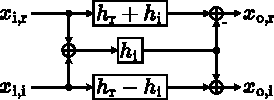
\includegraphics[keepaspectratio, scale=1]
                {\currfiledir/figs/mult_reduction_for_cplx_fd_fwd_flt.pdf}
                \caption{3 個の feedforward フィルタで実現された系}
            \end{figure}
    \section{CIC up-sampler}
    \label{CIC up-sampler}
    \newcommand*{\XNAF}{X_\text{NAF}}
    \newcommand*{\YNAF}{Y_\text{NAF}}
    \newcommand*{\tYNAF}{\tilde{Y}_\text{NAF}}
    \newcommand*{\XNF}{X_\text{NF}}
    \newcommand*{\YNF}{Y_\text{NF}}
    \newcommand*{\tYNF}{\tilde{Y}_\text{NF}}

    $R$ はアップ・サンプリング・レートを表し,$N$ は差分器と積算器それぞれの段数を表す。
    \par
    FPGA, ASIC による実装を前提として加算器(組み合わせ論理回路)の直後に Flip-flop を置く。
    Web 情報の多くはこれによる遅延を考慮しておらず,本書の結果と異なる数式を導いているが,影響があるのは遅延量だけであり,本質は変わらない。
    \subsection{周波数スペクトラム}
        \label{CIC up-sampler の周波数スペクトラム}
        差分器 1 つの漸化式は $y(n) = x(n-1) - x(n-2)$ であり,伝達関数は $(z^{-1})(1-z^{-1})$ である。
        ここに $x,y:\integers\to\complexNumbers$ は差分器への入力と出力である。
        同様に記号を流用して積算器の入出力 1 つの漸化式は $y(n) = y(n-1) + x(n-1)$ であり,伝達関数は $(z^{-1})/(1-z^{-1})$ である。
        Noble Identity を用いて $R$ 倍オーバー・サンプラを最前段に移動させると, $R$ 倍オーバー・サンプラの後ろの伝達関数は次式である。
        \[ H_\text{C,I}(z) = z^{-N(R+1)}\parens*{\frac{1-z^{-R}}{1-z^{-1}}}^N = z^{-N(R+1)}\parens*{\sum_{n=0}^{R-1} z^{-n}}^N \]
        これは,長さ $R$ の区間の和をとるブロックを $N$ 段従属接続して $N(R+1)$ だけ遅延させる操作と等価である。
        この系に対して $R$ 倍にオーバー・サンプルした結果を入力して得られる出力が CIC up-sampler の出力である。
        \par
        CIC up-sampler の出力の絶対値が最大となるのは,入力のビット幅が許す範囲の絶対値最大(この値を $x_\text{MAX}$ とおく)の定数列が入力された場合であり,値は次式である。
        \begin{equation}
            x_\text{MAX}R^{N-1}
            \label{equation:CIC up-sampler の出力の絶対値の最大値}
        \end{equation}
        このことから直ちに解るが, CIC up-sampler の直流ゲインは $R^{N-1}$ である。
        \par
        入力と出力の DTFT をそれぞれ $\XNAF(\Omega), \YNAF(\Omega)$ ($\Omega$ は正規化角周波数) とする。
        $H_\text{C,I}(z)$ に於いて $z = \exp(-i\Omega)$ とし,\ref{オーバー・サンプリングされた信号の DTFT} を適用し,周波数スペクトラムとして次式を得る。
        \begin{align*}
            \YNAF(\Omega) &= \exp(-iN(R+1)\Omega)\frac{\parens*{1-\exp\parens*{-iR\Omega}}^N}{R\parens*{1-\exp\parens*{-i\Omega}}^N}\XNAF(R\Omega) \\
            &= \exp\parens*{-i\frac{\Omega}{2}N(3R+1)}\parens*{\frac{\sin(R\Omega/2)}{\sin(\Omega/2)}}^N \XNAF(R\Omega)
        \end{align*}
        % ↓ 間違い。Noble Identity を用いて移動したオーバー・サンプラが区間和の 1 つと相殺することから勘違いした。ゲインが相殺するとはいえ,レートは元に戻らないのだから,完全に無視した式になるはずがない。
        % \begin{align*}
        %     \YNAF(\Omega) &= \exp(-iN(R+1)\Omega)\frac{\parens*{1-\exp\parens*{-iR\Omega}}^{N-1}}{\parens*{1-\exp\parens*{-i\Omega}}^{N-1}}\XNAF(R\Omega) \\
        %     &= \exp\parens*{-iN(R+1)\Omega}\exp\parens*{-i\frac{\Omega}{2}(N-1)(R-1)}\parens*{\frac{\sin(R\Omega/2)}{\sin(\Omega/2)}}^{N-1} \XNAF(R\Omega) \\
        %     &= \exp\exp\parens*{-i\frac{\Omega}{2}N(3R+1)}\parens*{\frac{\sin(R\Omega/2)}{\sin(\Omega/2)}}^{N-1} \XNAF(R\Omega)
        % \end{align*}
        正規化周波数で表現しなおして $\XNF(F) = \XNAF(2\pi F), \YNF(F) = \YNAF(2\pi F)$ とすれば次式を得る。
        \begin{align}
            \YNF(F) &= \exp\parens*{-i\frac{2\pi F}{2}N(R-1)}\parens*{\frac{\sin(R 2\pi F/2)}{\sin(2\pi F/2)}}^N \XNF(R F) \nonumber \\
            &= \exp\parens*{-i\pi N(3R+1)F}\parens*{\frac{\sin(\pi R F)}{\sin(\pi F)}}^N \XNF(R F) \label{equation:CIC up-sampler の周波数スペクトラム}
        \end{align}
        この式は $F\to 0$の極限で $R^N \XNF(0)$ となる。
        しかし入力を直流としたときに出力の絶対値が $R^N$ 倍になるわけではない。
        なぜならば既に述べたように, Noble Identity を用いて移動したオーバー・サンプラが,伝達関数に含まれる長さ $R$ の区間和の 1 つと相殺するからである。
        周波数スペクトラムと「振幅特性」(すぐ後に明かされるように,この単語は正しく定義されないので敢えて「」付きで示した)が一致しない原因は単純で,オーバー・サンプルという非線形な操作を加えた結果,正弦波入力に対する出力が正弦波とならないからである。
        この状況では「振幅特性」自体が定義できない。
        アップ・サンプルによって正弦波が緻密になって出力されたように見えても,それは「そう見える」だけであり,厳密には正弦波ではなく広がりをもったスペクトラムをもつ信号に変わっている。
    \subsection{差分器と積算器に必要なビット幅}
        \subsubsection{差分器のビット幅}
            差分器の出力の絶対値が最大となるのは,入力のビット幅が許す範囲の最大振幅の交代列が入力された場合である。
            よって,差分器の出力のビット幅は入力のそれの 2 倍を確保すればよく,$N$ 段目の差分器の出力のビット幅は初段の入力のビット幅 + $N$ とすればよい。
        \subsubsection{積算器のビット幅(解析的な方法)}
            CIC up-sampler の入力のビット幅を $B$ とする。
            まず,\cref{equation:CIC up-sampler の出力の絶対値の最大値} より最終段の積算器(第 $N$ 積算器)の出力のビット幅は $B + (N-1)\log_2 R$ を確保すれば必要十分である。
            \par
            最終段より前の積算器については必要十分なビット幅を解析的に求めることはできないが,十分な値であれば次のようにして求められる。
            \par
            第 $(N-1)$ 積算器の出力のビット幅を考える。
            第 $2$ 差分器から第 $(N-1)$ 積算器までに注目すると,これはステージ数 $N-1$ の CIC up-sampler となっている。
            このことと,元の第 $1$ 差分器の出力の絶対値の最大値がビット幅 $B+1$ で収容できることから,第 $(N-1)$ 積算器の出力はビット幅 $B + 1 + (N-2)\log_2 R$ を確保すれば十分である。
            (元の第 $1$ 差分器の出力が最大値で一定していることはあり得ないことは容易に解る。
            この点を無視して上限で評価しており,故に「必要な」ビット幅からの乖離がある。)
            \par
            同様にして次々に内側の小さい CIC up-sampler を考えてゆくと,十分なビット幅が求まる。
        \subsubsection{積算器のビット幅(数値的な方法)}
            最終段については既に述べたように解析的に求められるのでここでは扱わない。
            \par
            Noble Identity を用いて $R$ 倍オーバー・サンプラを最前段に移動した後,第 1 差分器から第 $n\in\{1,2,...,N-1\}$ 段の積算器までの部分系の伝達関数を考えると次式を得る。
            \[ \frac{(1-z^{-R})^N}{(1-z^{-1})^n} = (1-z^{-R})^{N-n}\parens*{\sum_{n=0}^{R-1} z^{-n}}^n \]
            上式のうち,$\sum_{n=0}^{R-1} z^{-n}$ 1つ分については,この系の前段に移動された $R$ 倍オーバー・サンプラと相殺し,ビット幅増加に寄与しない。
            よって,ビット幅の増加に寄与する部分は次式である。
            \begin{equation}
                \frac{(1-z^{-R})^N}{(1-z^{-1})^n} = (1-z^{-R})^{N-n}\parens*{\sum_{n=0}^{R-1} z^{-n}}^{n-1} \label{equation:CIC up-sampler の部分系の伝達関数}
            \end{equation}
            これは抽出された部分系の有限インパルス応答の z 変換である。
            この系の応答の絶対値が最大となるような作為的な入力に対する応答を収容できるビット幅を確保すればよい。
            そのような最悪の応答は \cref{equation:CIC up-sampler の部分系の伝達関数} を計算機代数システムを用いて $z^{-1}$ の多項式として展開し,係数の絶対値の総和をとることで得られる。
    \subsection{CIC up-sampler 補償フィルタ}
        \newcommand*{\HCNF}{H_\text{C,NF}}

        \cref{equation:CIC up-sampler の周波数スペクトラム} より,アップ・サンプリングにより $\XNF$ には $F$ に依存する因子が掛かる。
        これをできるだけ補正するために,CIC up-sampler の直前で前記の因子の逆特性を近似する feedforward フィルタ(以下単に「FIR フィルタ」と呼ぶ)の適用を考える($F$ に依存しないスケーリング因子 $1/R$ は容易に補正できるので,今は無視する)。
        このフィルタの周波数スペクトラムを $\HCNF$ とすると次式が成り立つ。
        \[ \YNF(F) = \exp\parens*{-i\pi N(3R+1)F}\parens*{\frac{\sin(\pi R F)}{\sin(\pi F)}}^N \HCNF(R F)\XNF(R F) \]
        $\HCNF(F)$ に求められるのは $F \in [-1/2,1/2]$ の範囲で次式を近似することである。
        \begin{equation}
            \exp\parens*{i\pi N\frac{R-1}{R}F}\parens*{\frac{\sin(\pi F/R)}{\sin(\pi F)}}^N \label{equation:CIC up-sampler 補償フィルタの理想的な周波数スペクトラム}
        \end{equation}
        $R$ が大きいとき,$\sin(\pi F/R) \sim \pi F/R$ として \cref{equation:CIC up-sampler 補償フィルタの理想的な周波数スペクトラム} の振幅特性が(Fに依存しないスケールの違いを除いて) $1/\sinc(\pi F)^N$ に漸近する。
        \par
        $\HCNF$ が周期 1 の関数であることから, $[-1/2,1/2]$ の区間全体で上式を近似することはできない(端点で微分不可能になる)。
        現実には,$\alpha[-1/2,1/2]\;(0<\alpha<1)$ の範囲を Remez のアルゴリズム等で近似する。
        $\alpha$ が 1 に近づく程,必要な係数が増える。
        \cref{equation:CIC up-sampler の周波数スペクトラム} が示すように CIC up-sampler の位相特性が線形なので Remez のアルゴリズムでは振幅の補正だけを気にして係数設計してよい(生成される feedforward フィルタ(以下単に「FIR フィルタ」と呼ぶ)の位相特性も線形なので合成系の位相特性も線形となる)。
        \par
        アップ・サンプリングを全て CIC up-sampler で行うのではなく,一部を CIC up-sampler の前段のゼロ埋めと FIR フィルタ(「FIR フィルタ 1」と呼ぶ)に分担させ,そのフィルタに後段の CIC up-sampler の補正フィルタを兼任させる(合成する)こともしばしば行われる。
        例えば, FIR フィルタ 1 の直前で x2 zero-padding を行う場合,フィルタ 1 では $0.8\times[-1/4,1/4]$ の領域で \cref{equation:CIC up-sampler 補償フィルタの理想的な周波数スペクトラム} を近似し,$[-1/2,-1/2+0.8/4]\cup[1/2-0.8/4,1/2]$ の領域を阻止帯とするように Remez のアルゴリズムで係数を計算する。
\section{CIC down-sampler}
    $R$ はダウン・サンプリング・レートを表し,$N$ は差分器と積算器それぞれの段数を表す。
    \ref{CIC up-sampler} と同様に加算器(組み合わせ論理回路)の直後に Flip-flop を置く。
    \subsection{周波数スペクトラム}
        Noble Identity を用いて $R$ 倍アンダー・サンプラを最終段に移動させると,\ref{CIC up-sampler の周波数スペクトラム} と同様にして, $1/R$ 倍アンダー・サンプラより前の伝達関数は次式である。
        \[ H_\text{I,C}(z) = z^{-N(R+1)}\parens*{\frac{1-z^{-R}}{1-z^{-1}}}^N = z^{-N(R+1)}\parens*{\sum_{n=0}^{R-1}z^{-n}}^N \]
        これは,長さ $R$ の区間の和をとるブロックを $N$ 段従属接続して $N(R+1)$ だけ遅延させる操作と等価である。
        この系の出力を 1/R でサンプリングした結果が CIC down-sampler の出力である。
        よって,系の出力の絶対値が最大となるのは,絶対値が最大の定数 ($x_\text{MAX}$ とする)を入力し続けたときであり,そのときの出力の絶対値は $R^N x_\text{MAX}$ である。
        このことから直ちに解るが,直流ゲインは $R^N$ である。
        \par
        入力の DTFT を $\XNAF(\Omega)$ ($\Omega$ は正規化角周波数) とする。
        $1/R$ 倍アンダー・サンプラより前の出力の DTFT を $\tYNAF(\Omega)$ とする。
        $H_\text{I,C}(z)$ に於いて $z = \exp(-i\Omega)$ とすると次式が成り立つ。
        \begin{align*}
            \tYNAF(\Omega) &= \exp(-iN(R+1)\Omega)\frac{\parens*{1-\exp\parens*{-iR\Omega}}^N}{\parens*{1-\exp\parens*{-i\Omega}}^N}\XNAF(\Omega) \\
            &= \exp\parens*{-i\frac{\Omega}{2}N(3R+1)}\parens*{\frac{\sin(R\Omega/2)}{\sin(\Omega/2)}}^N \XNAF(\Omega)
        \end{align*}
        正規化周波数で表現しなおして $\XNF(F) = X(2\pi F), \tYNF(F) = \tYNAF(2\pi F)$ とすれば次式を得る。
        \[ \tYNF(F) = \exp\parens*{-i\pi N(3R+1)F}\parens*{\frac{\sin(\pi R F)}{\sin(\pi F)}}^N \XNF(F) \]
        これと \ref{アンダー・サンプリングされた信号の DTFT} より,$1/R$ 倍アンダー・サンプラの出力を正規化周波数で表現した周波数スペクトラムは次式である。
        \begin{align}
            \YNF(F) &= \frac{1}{R}\sum_{n=0}^{R-1} \tYNF((F-n)/R) \nonumber \\
            &= \frac{1}{R}\sum_{n=0}^{R-1} \exp\parens*{-i\pi N(F-n)(3R+1)/R}\parens*{\frac{\sin(\pi(F-n))}{\sin(\pi(F-n)/R)}}^N \XNF((F-n)/R) \label{equation:CIC down-sampler の周波数スペクトラム}
        \end{align}
        \ref{アンダー・サンプリングされた信号の DTFT} でも述べられているが,全体に掛けられている $1/R$ は DTFT の内積計算の対象となる点の数が $1/R$ に減ったことに由来しており,振幅が $1/R$ になるわけではない。
    \subsection{差分器と積算器に必要なビット幅}
        入力は固定小数点数であるが,全体を適当に2のべき乗倍したものとして見直して符号付整数として扱っても系としては等価なので,以後そうする。
        入力側(サンプル・レートが高い側)から入力される符号付整数のビット幅を $B$ とする。
        \par
        先の議論から,最終段の出力のビット幅は $\ceil{1 + \log_2\parens{R^N 2^{B-1}}} = B + \ceil{N\log_2 R}$ あれば十分であることが判る。
        \par
        積算器はオーバー・フローし得るが,溢れた桁を捨てる操作が modulo 演算であることと,最終段の出力のビット幅を考えれば,最終段より左側の全ての段のビット幅を最終段と等しくしておけば問題ない(無限のビット幅を持つ仮想的な系と同じ出力が得られる)ことが判る。
    \subsection{CIC down-sampler 補償フィルタ}
        \cref{equation:CIC down-sampler の周波数スペクトラム} より,ダウン・サンプリングにより $\XNF$ には $F$ に依存する因子が掛かる。
        これをできるだけ補正するために,CIC down-sampler の直後で前記の因子の逆特性を近似する feedforward フィルタの適用を考える($F$ に依存しないスケーリング因子 $1/R$ は容易に補正できるので,今は無視する)。
        ダウン・サンプリング後に補償用フィルタを掛けるので第 1 Nyquist 領域のみに関心を払えばよい(とうより,それを超えてできることはない)。
        第 1 Nyquist 領域のみを抽出し,補償用フィルタの周波数スペクトラムを $\HCNF$ とすると次式が成り立つ。
        \[ \YNF(F) = \HCNF(F) \frac{1}{R} \exp\parens*{-i\pi N F(3R+1)/R}\parens*{\frac{\sin(\pi F)}{\sin(\pi F/R)}}^N \XNF(F/R) \]
        $\HCNF(F)$ に求められるのは $F \in [-1/2,1/2]$ の範囲で次式を近似することである。
        \begin{equation}
            \exp\parens*{i\pi N F(3R+1)/R}\parens*{\frac{\sin(\pi F/R)}{\sin(\pi F)}}^N
        \end{equation}
        この式は偏角の差を除いて \cref{equation:CIC up-sampler 補償フィルタの理想的な周波数スペクトラム} と一致するため,補償用フィルタの設計手法は CIC up-sampler 補償フィルタと同じものを適用できる。

